\documentclass[a4paper,12pt,oneside]{book}
\usepackage[T1]{fontenc}                                      
\usepackage[utf8]{inputenc}                               
\usepackage[italian]{babel}
\usepackage{amsfonts}
\usepackage{amsthm}
\usepackage{amsmath,amssymb}
\usepackage{array}
\usepackage{arydshln}
\usepackage{braket}
\usepackage{blindtext}
\usepackage{calc}
\usepackage{cancel}
\usepackage{caption}
\usepackage{epsfig}
\usepackage{eucal}
\usepackage{fancyhdr}
\usepackage{geometry}
\usepackage{graphicx}
\usepackage{indentfirst}
\usepackage{hhline}
\usepackage{hyperref}
\hypersetup{
			colorlinks=true,
			linkcolor=black,
			anchorcolor=black,
			citecolor=black,
			urlcolor=black,
			pdftitle={Appunti di Meccanica Quantistica},
			pdfauthor={Vittorio Lubicz}
}

\usepackage{latexsym}
\usepackage{listings} 
\usepackage{longtable}
\usepackage{makeidx}
\usepackage{mathrsfs}
\usepackage{mathdots}
\usepackage{multirow}
\usepackage{nicefrac}
\usepackage{pdfpages}
\usepackage{physics}
\usepackage{setspace}
\usepackage{tikz}
\usepackage{tikz-3dplot}
\usepackage{textcomp}
\usepackage{titlesec,color}
\usepackage{vmargin}
\setpapersize{A4}
\setmarginsrb{35mm}{30mm}{35mm}{30mm}%
             {0mm}{10mm}{0mm}{10mm}



\definecolor{gray75}{gray}{0.75}
\newcommand{\hsp}{\hspace{20pt}}

\titleformat{\chapter}[hang]{\huge\bfseries}{\myfont{\textit{\large{\chaptername\hspace{1pt} \thechapter\hspace{3pt}}}}\textcolor{gray75}{$\mid$}\hspace{0.4cm}}{0pt}{\myfont{\huge\bfseries}}

\titleformat{\section}[hang]{\large\bfseries}{\myfont{\textit{\normalsize{\thesection\hspace{2pt}}}}\hspace{0.4cm}}{0pt}{\myfont{\Huge\bfseries}}

\titleformat{\subsection}[hang]{\large\bfseries}{\myfont{\textit{\small{\thesubsection\hspace{2pt}}}}\hspace{0.4cm}}{0pt}{\myfont{\huge\bfseries}}

\renewcommand{\chaptermark}[1]{\markboth{#1}{}}
\renewcommand{\sectionmark}[1]{\markright{#1}}
\newcommand*{\myfont}{\fontfamily{ppl}\selectfont}

\begin{document}

%*****************LAYOUT PAGINE**************************
\fancypagestyle{plain}{%
\fancyhf{} % cancella tutti i campi di  intestazione e pi\`e di pagina
\fancyfoot[C]{\bfseries \myfont{\thepage}} % tranne il centro
\renewcommand{\headrulewidth}{0pt}
\renewcommand{\footrulewidth}{0pt}}

\fancypagestyle{VS}{
\headheight = 15pt
\lhead[\myfont{\textit{\textbf{\thechapter\nouppercase{\leftmark}}}}]{\myfont{\textit{\textbf{\nouppercase{\leftmark}}}}}
\chead[]{}
\rhead[\myfont{\textbf{\thepage}}]{\myfont{\textbf{\thepage}}}

\lfoot[]{}
\cfoot[]{}
\rfoot[]{}
}
%*******************************************************



\pagestyle{VS}
\setcounter{chapter}{24}
\setcounter{page}{238}
\chapter[Correzioni relativistiche all'atomo di idrogeno]{Correzioni relativistiche\\ all'hamiltoniano\\ dell'atomo di idrogeno\footnote{G17, S5.3}}

La trattazione fatta dell'atomo di idrogeno era basata sull'hamiltoniana
\begin{equation} \label{eq:cap25_1}
H_0=\frac{\vec{p^2}}{2m}-\frac{\mathcal{Z} e^2}{r}
\end{equation}
($\mathcal{Z}=1$ per l'atomo di idrogeno). In una trattazione più realistica è necessario prendere in considerazione diverse \textbf{correzioni}.

\section{Termine cinetico}

L'espressione dell'\textbf{energia cinetica} dell'elettrone si modifica quando si considerano \textbf{correzioni relativistiche }. Nella meccanica relativistica l'energia cinetica è data da:

\begin{eqnarray} 
E & = &\sqrt{m^2c^4+c^2\vec{p^2}}= mc^2 \sqrt{1+ \frac{\vec{p^2}}{m^2c^2}} \simeq \nonumber  \\
& \simeq & mc^2 \left( 1+ \frac{\vec{p^2}}{2m^2c^2}-\frac{(\vec{p^2})^2}{8m^4c^4}+\dots \right) = \nonumber  \\
& = & mc^2+\frac{\vec{p^2}}{2m}-\frac{(\vec{p^2})^2}{8m^3c^2}+ \dots 
\end{eqnarray}
Il termine della massa a riposo rappresenta una costante additiva irrilevante nella definizione dell'energia. La prima correzione relativistica è allora data dal termine 
\begin{equation} \label{eq:cap25_2}
H_1=-\frac{(\vec{p^2})^2}{8m^3c^2} ,
\end{equation}
che deve essere aggiunto all'hamiltoniana $H_0$. \\
Una stima dell'effetto di questa correzione sui livelli di energia dell'atomo può essere ottenuto utilizzando il principio di indeterminazione ed assumendo come valore approssimato del raggio dell'orbita \textbf{elettronica il valore $\boldsymbol{a_0\mathcal{Z}}$}. Si ottiene in tal modo
\begin{equation} 
\frac{\left< H_1 \right>}{\langle H_0 \rangle} \approx \frac{\vec{p^2}}{m^2c^2} \simeq \frac{\hbar^2 \mathcal{Z}^2}{m^2c^2a_0^2}=\frac{\mathcal{Z}^2 \hbar^2}{m^2c^2} \left( \frac{me^2}{\hbar^2}\right)^2=\frac{\mathcal{Z}^2 e^4}{\hbar^2 c^2} ,
\end{equation}
ossia
\begin{equation} 
\frac{\left< H_1 \right>}{\langle H_0 \rangle} \approx \left( \frac{v_e}{c} \right)^2 \approx \left(  \mathcal{Z} \alpha \right)^2 ,
\end{equation}
dove
\begin{equation} 
\alpha=\frac{e^2}{\hbar c} \simeq \frac{1}{137}
\end{equation}
è la cosiddetta costante di struttura fine. \\ Così, per l'atomo di idrogeno, questa correzione relativistica è dell'ordine di grandezza relativo di $\sim10^{-4}$.
\section{Accoppiamento spin-orbita}

L'\textbf{esistenza dello spin} dell'elettrone implica un'altra \textbf{correzione dello stesso ordine di grandezza}. Questa può essere qualitativamente compresa col seguente ragionamento: se l'elettrone fosse in quiete rispetto al protone, risentirebbe solo di un campo elettrico generato dalla carica del protone. Questo è il \textbf{termine del potenziale di Coulomb che appare in $\boldsymbol{H_0}$}. Poiché l'elettrone è però in movimento vi sono effetti addizionali. \\
\textbf{Nel sistema di riferimento dell'elettrone, il protone è in moto così che è presente una corrente e l'elettrone risente di un campo magnetico. Questo campo magnetico interagisce con lo spin dell'elettrone, o, più precisamente, con il momento magnetico dell'elettrone}. \\
Se il moto relativo del protone rispetto all'elettrone fosse rettilineo, il campo magnetico visto dall'elettrone sarebbe dato da:
\begin{equation} 
\vec{B}^{'}=-\gamma \frac{\vec{v}}{c} \wedge \vec{E} \ \simeq -\frac{\vec{v}}{c} \wedge \vec{E} ,
\end{equation}
dove $\vec{E}$ è il campo elettrico nel sistema di quiete del protone. \\
Poiché l'elettrone ha un momento magnetico intrinseco proporzionale al suo spin, dalla forma
\begin{equation} 
\vec{\mu}=-\frac{e}{mc}\vec{S} 
\end{equation}
ci aspettiamo che l'interazione con il campo magnetico effettivo risulti data da
\begin{eqnarray}
H_2 & =& -\vec{\mu} \cdot \vec{B}^{'}=\frac{e}{mc} \vec{S} \cdot \vec{B}^{'}= -\frac{e}{mc^2}\vec{S} \cdot \left( \vec{v} \wedge \vec{E} \right)= \nonumber \\
& =& + \frac{e}{m^2c^2}\vec{S} \cdot \vec{p} \wedge \vec{\nabla}\phi= \frac{e}{m^2c^2}\vec{S} \cdot \vec{p} \wedge \frac{\vec{r}}{r} \ \frac{d\phi}{dr}= \nonumber \\
& = &-\frac{e}{m^2c^2}\frac{1}{r} \ \frac{d\phi}{dr}\vec{S} \cdot \vec{L}= \frac{1}{m^2c^2} \left( \frac{1}{r} \ \frac{dV}{dr} \right) \vec{S} \cdot \vec{L} ,
\end{eqnarray}

dove $V=-e\phi=-\mathcal{Z}e^2/r$ è il potenziale cui è soggetto l'elettrone. \\
In realtà il moto dell'elettrone non è rettilineo uniforme, ed il risultato ottenuto risulta troppo grande di un fattore $2$ (\textbf{questo effetto è noto come precessione di Thomas}. Il termine di interazione corretto ha dunque la forma
\begin{equation} \label{eq:cap25_3}
H_2=\frac{1}{2m^2c^2} \left( \frac{1}{r} \ \frac{dV}{dr} \right) \vec{S} \cdot \vec{L} ,
\end{equation}
con
\begin{equation} 
V=-\frac{\mathcal{Z}e^2}{r} .
\end{equation}
Anche in questo caso è semplice ottenere una \textbf{stima della correzione} indotta dal termine aggiuntivo nell'hamiltoniana:
\begin{eqnarray}
\frac{\left< H_2 \right>}{\langle H_0 \rangle} & \approx & \frac{1}{m^2c^2} \left( \frac{1}{r} \ \frac{\mathcal{Z}e^2}{r^2} \right) \vec{S} \cdot \vec{L} \cdot \left( \frac{\mathcal{Z}e^2}{r} \right)^{-1} \approx \nonumber  \\
& \approx &\frac{\vec{S} \cdot \vec{L}}{m^2c^2r^2} \approx  \frac{\hbar^2 \mathcal{Z}^2}{m^2c^2a_0^2}=  \frac{\mathcal{Z}^2 \hbar^2}{m^2c^2}\left( \frac{me^2}{\hbar^2} \right)^2= \frac{\mathcal{Z}^2e^4}{\hbar^2c^2} ,
\end{eqnarray}
ossia
\begin{equation} 
\frac{\left< H_2 \right>}{\langle H_0 \rangle} \approx \left( \mathcal{Z}\alpha \right)^2 .
\end{equation}
L'interazione spin-orbita induce pertanto una correzione relativa ai livelli energetici dell'atomo che è dello stesso ordine di grandezza della correzione relativistica dovuta al termine cinematico ($\sim10^{-4}$ per $\mathcal{Z}=1$).
\section{Calcolo perturbativo delle correzioni}

L'effetto stimato delle correzioni ai livelli energetici degli atomo idrogenoidi, indotto dalla correzione relativistica all'energia cinetica e dell'accoppiamento spin-orbita, è sufficientemente piccolo da poter essere trattato, con ottima approssimazione, nella \textbf{teoria delle perturbazioni}. \\
Consideriamo come hamiltoniana imperturbata l'hamiltoniana $H_0$ dell'equazione (\ref{eq:cap25_1}) e come perturbazione $V$ la somma delle hamiltoniane $H_1$ e $H_2$ definite in equazione (\ref{eq:cap25_2}) e (\ref{eq:cap25_3}):
\begin{equation} 
V=H_1+H_2=-\frac{p^4}{8m^3c^2}+\frac{1}{2m^2c^2} \left( \frac{1}{r} \ \frac{dV}{dr} \right) \vec{S} \cdot \vec{L} .
\end{equation}
Proponiamoci qui di calcolare le \textbf{correzioni ai livelli energetici imperturbati, al primo ordine nella perturbazione $\boldsymbol{V}$}. \\
I livelli di energia dell'hamiltoniana imperturbata $H_0$, corrispondenti ad un determinato valore del numero quantico principale $n$, hanno un grado di degenerazione pari a $2n^2$. Gli stati degeneri differiscono per i diversi valori dei numeri quantici $l,m_l$ ed $m_s$ definiti dagli autovalori di $L^2$, $L_z$ ed $S_z$. Per tutti gli stati con $n>1$ risulta quindi necessario applicare la \textbf{teoria delle perturbazioni nel caso degenere}. \\
Il calcolo risulta estremamente semplificato se, per quanto concerne la dipendenza delle variabili angolari e di spin delle funzioni d'onda imperturbate, si considerano gli \textbf{autostati di}
\begin{equation} \label{eq:cap25_4}
J^2, \ J_x, \ L^2, \ S^2 ,
\end{equation}
in luogo degli autostati di $L^2, L_z, S^2, S_z$. \\
Le perturbazioni $H_1$ ed $H_2$ possono infatti essere scritte convenientemente nella forma
\begin{equation} \label{eq:cap25_5}
H_1=-\frac{1}{2mc^2} \left( \frac{\vec{p^2}}{2m} \right)^2 = -\frac{1}{2mc^2} \left( H_0+\frac{\mathcal{Z}e^2}{r} \right)^2 ,
\end{equation}
e
\begin{equation} \label{eq:cap25_6}
H_2=\frac{1}{4m^2c^2} \left( \frac{1}{r} \ \frac{dV}{dr} \right) \left(\vec{J}^2-\vec{L}^2-\vec{S}^2 \right) .
\end{equation}
Da queste espressioni risulta infatti evidente che \textbf{gli operatori $\boldsymbol{H_1}$ ed $\boldsymbol{H_2}$ commutano con gli operatori in equazione (\ref{eq:cap25_4}), cosicché, nella corrispondente base, la perturbazione risulta già diagonale}. \\ (\'E bene sottolineare, tuttavia, che le perturbazioni $H_1$ ed $H_2$ non commutano, ovviamente, con l'hamiltoniano imperturbato $H_0$. Pertanto $H_1$ ed $H_2$ risultano diagonali solo nel sottospazio degli autostati degeneri di $H_0$ corrispondenti a diversi valori di $J^2$, $J_z$ ed $L^2$). \\
\textbf{Le correzioni al primo ordine ai livelli energetici dell'atomo si ottengono allora direttamente calcolando i valori di aspettazione della perturbazione $\boldsymbol{V}$ sugli autostati di $\boldsymbol{H_0}$, $\boldsymbol{J^2}$, $\boldsymbol{J_z}$, $\boldsymbol{L^2}$, $\boldsymbol{S^2}$}. \textbf{Indichiamo questi autostati con}
\begin{equation} 
| n,l,j,m_j \rangle .
\end{equation}
Per un determinato valore del numero quantico orbitale $l$, il numero quantico $j$ può assumere i valori
\begin{equation} 
j=l\pm1/2 .
\end{equation}
Le corrispondenti autofunzioni sono della forma
\begin{equation} 
\psi_{n,l,j,m_j}=R_{nl}(r)Y_{j=l\pm1/2,m_j} .
\end{equation}
Cominciamo con il calcolare, su questi stati, \textbf{i valori medi della perturbazione $\boldsymbol{H_1}$} indotta dalle correzioni relativistiche all'energia cinetica. Utilizziamo l'equazione ($\ref{eq:cap25_5}$) troviamo:
\begin{eqnarray} \label{eq:cap25_7} 
& &\langle n,l,j,m_j | H_1 |n,l,j,m_j \rangle = \nonumber \\
& &=-\frac{1}{2mc^2}\langle n,l,j,m_j |\left( H_0+\frac{\mathcal{Z}e^2}{r} \right) \left( H_0+\frac{\mathcal{Z}e^2}{r} \right)  |n,l,j,m_j \rangle = \nonumber \\
& &=-\frac{1}{2mc^2}\langle n,l,j,m_j | \left( E_n+\frac{\mathcal{Z}e^2}{r} \right)^2  | n,l,j,m_j\rangle = \nonumber \\
& &=-\frac{1}{2mc^2} \left( E_n^2+2E_n\mathcal{Z}e^2 \left< \frac{1}{r} \right>_{nl} +\left( \mathcal{Z}e^2 \right)^2\left< \frac{1}{r^2} \right>_{nl} \right)  ,
\end{eqnarray}
dove si sono definiti i valori medi
\begin{eqnarray} 
\left< \frac{1}{r^k} \right>_{nl} & = \langle n,l,j,m_j | \frac{1}{r^k} | n,l,j,m_j \rangle = \nonumber\\
& = \int_0^{\infty} dr \ r^2 \ \frac{1}{r^k} \left( R_{nl}(r) \right)^2 .
\end{eqnarray}
Per questi valori medi sono note delle formule generali, che qui riportiamo:
\begin{equation} \label{eq:cap25_8}
\begin{split}
\left< \frac{1}{r} \right>_{nl} & = \left( \frac{\mathcal{Z}}{a_0} \right) \frac{1}{n^2} , \\ 
\left< \frac{1}{r^2} \right>_{nl} & = \left( \frac{\mathcal{Z}}{a_0} \right)^2 \frac{1}{n^3(l+1/2)}  ,\\ 
\left< \frac{1}{r^3} \right>_{nl} &= \left( \frac{\mathcal{Z}}{a_0} \right)^3 \frac{1}{n^3 \ l \ (l+1/2)(l+1)} \qquad (l \neq0) .
\end{split}
\end{equation}
(Il valor medio $\left<1/r^3\right>_{nl}$ risulterà utile nel calcolo della correzione indotta dall'accoppiamento spin-orbita). \\
Sostituendo i valori medi (\ref{eq:cap25_8}) nell'equazione (\ref{eq:cap25_7}) ed utilizzando le espressioni
\begin{equation} 
E_n=-\frac{mc^2 \left(\mathcal{Z}\alpha\right)^2}{2n^2} 
\end{equation}
per l'energia dei livelli imperturbati e 
\begin{equation} 
a_0=\frac{\hbar^2}{me^2}=\frac{\hbar^2c^2}{e^4}\frac{e^2}{mc^2}=\frac{e^2}{mc^2\alpha^2}
\end{equation}
per il raggio di Bohr, otteniamo:

\begin{eqnarray} 
 \left< H_1 \right>_{nljm_j} & =& -\frac{1}{2mc^2} \left[ \frac{m^2c^4 \left( \mathcal{Z} \alpha \right)^4}{4n^4}-\frac{mc^2 \left( \mathcal{Z} \alpha \right)^2 \mathcal{Z} e^2}{n^4} \frac{mc^2\alpha^2 \mathcal{Z}}{e^2}+ \right. \nonumber \\
& &\left. + \left( \mathcal{Z} e^2 \right)^2 \frac{1}{n^3(l+1/2)} \left(\frac{mc^2\alpha^2}{e^2} \right)^2 \mathcal{Z}^2 \right] = \nonumber  \\
& = & -\frac{1}{2mc^2} \left( m^2c^4 \right) \left( \mathcal{Z} \alpha\right)^4 \left[ \frac{1}{4n^4}-\frac{1}{n^4}+\frac{1}{n^3(l+1/2)}  \right] ,
\end{eqnarray}
ossia
\begin{equation} \label{eq:cap25_9}
\left< H_1 \right>_{nljm_j} = -\frac{1}{2}mc^2 \left( \mathcal{Z} \alpha \right)^4 \left[ \frac{1}{n^3(l+1/2)}-\frac{3}{4n^4}\right]  .
\end{equation}
Questa correzione risulta dall'ordine di grandezza aspettato: più piccola di circa un fattore $\left( \mathcal{Z} \alpha \right)^2$ rispetto ai livelli di energia imperturbati. \\
Calcoliamo ora la \textbf{correzione}, al primo ordine dello sviluppo perturbativo, \textbf{indotto} sui livelli di energia imperturbati \textbf{dall'interazione spin-orbita}. \\ 
Utilizzando l'equazione (\ref{eq:cap25_6}) otteniamo:
\begin{eqnarray} \label{eq:cap25_10}
\left< H_2 \right>_{nljm_j} &=& \langle n,l,j,m_j | H_2 | n,l,j,m_j \rangle = \nonumber  \\
& = &\frac{1}{4m^2c^2} \langle n,l,j,m_j | \left( \frac{\mathcal{Z}e^2}{r^3} \right) \left( \vec{J}^2-\vec{L}^2-\vec{S}^2 \right)      | n,l,j,m_j \rangle= \nonumber  \\
& = & \frac{\hbar^2\mathcal{Z}e^2}{4m^2c^2} \left< \frac{1}{r^3} \right>_{nl} \left[ j(j+1)-l(l+1)-\frac{3}{4}  \right] .
\end{eqnarray}
Il fattore tra parentesi quadre che entra in questa espressione, nei due casi $j=l\pm1/2$, vale 
\begin{eqnarray} 
& &\left. \left[ j(j+1)-l(l+1)-\frac{3}{4}  \right]  \right|_{j=l+1/2} = \nonumber \\ 
& &\qquad = \left( l+\frac{1}{2} \right) \left( l+\frac{3}{2}\right)-l\left(l+1 \right) -\frac{3}{4}=l
\end{eqnarray}
e
\begin{eqnarray} 
& &\left. \left[ j(j+1)-l(l+1)-\frac{3}{4}  \right] \right|_{j=l-1/2} = \nonumber  \\ 
& &\qquad = \left( l-\frac{1}{2} \right) \left(l+\frac{1}{2} \right)-l\left( l+1 \right) -\frac{3}{4}=-l-1 .
\end{eqnarray}
Sostituendo questi risultati nell'equazione (\ref{eq:cap25_10}), insieme al valore medio $\left< 1/r^3 \right>_{nl}$ dato nell'equazione (\ref{eq:cap25_8}), si ottiene:
\begin{equation} \label{eq:cap25_11}
\left< H_2 \right>_{nljm_j}=\frac{1}{4}mc^2\left( \mathcal{Z}\alpha \right)^4 \frac{\begin{Bmatrix}
      l  \\ 
      -l-1 
    \end{Bmatrix}
    \begin{matrix}
    \leftarrow j=l+1/2 \\
    \leftarrow j=l-1/2
    \end{matrix} }{n^3 \ l \ \left(l+1/2 \right) \left( l+1 \right)} ,
\end{equation}
valida per $l\neq0$. La correzione è nulla per $l=0$. \\
Le due correzioni, fornite dalle equazioni (\ref{eq:cap25_9}) e (\ref{eq:cap25_11}), possono essere infine combinate per ottenere la \textbf{correzione totale}, al primo ordine nella perturbazione, ai livelli di energia degli atomi idrogenoidi. Nei due casi, corrispondenti a $j=l\pm1/2$ si ottiene:

\begin{eqnarray} 
\left( \Delta E \right)_{j=l+1/2} &= & \left( \left< H_1\right> +\left<H_2 \right>  \right)_{j=l+1/2}= \nonumber \\
& =& -\frac{1}{2} mc^2 \left( \mathcal{Z}\alpha \right)^4 \frac{1}{n^3} \left[ \frac{1}{l+1/2}-\frac{3}{4n}-\frac{1}{2(l+1/2)(l+1)}\right]=  \nonumber \\
& = & -\frac{1}{2} mc^2 \left( \mathcal{Z}\alpha \right)^4 \frac{1}{n^3} \left[ \frac{l+1-1/2}{(l+1/2)(l+1)}-\frac{3}{4n}\right]= \nonumber  \\
& =v& -\frac{1}{2} mc^2 \left( \mathcal{Z}\alpha \right)^4 \frac{1}{n^3} \left[ \frac{1}{l+1}-\frac{3}{4n} \right]= \nonumber \\
& = &-\frac{1}{2} mc^2 \left( \mathcal{Z}\alpha \right)^4 \frac{1}{n^3} \left[ \frac{1}{j+1/2}-\frac{3}{4n} \right]
\end{eqnarray}
e
\begin{eqnarray} 
 \left( \Delta E \right)_{j=l-1/2}&=&\left( \left< H_1\right> +\left<H_2 \right>  \right)_{j=l-1/2}= \nonumber \\
& = &-\frac{1}{2} mc^2 \left( \mathcal{Z}\alpha \right)^4 \frac{1}{n^3} \left[ \frac{1}{l+1/2}-\frac{3}{4n}-\frac{1}{2l(l+1/2)}\right]= \nonumber \\
& =& -\frac{1}{2} mc^2 \left( \mathcal{Z}\alpha \right)^4 \frac{1}{n^3} \left[ \frac{l+1/2}{l(l+1/2)}-\frac{3}{4n}\right]= \nonumber \\
& = &-\frac{1}{2} mc^2 \left( \mathcal{Z}\alpha \right)^4 \frac{1}{n^3} \left[ \frac{1}{l}-\frac{3}{4n} \right]= \nonumber  \\
& = & -\frac{1}{2} mc^2 \left( \mathcal{Z}\alpha \right)^4 \frac{1}{n^3} \left[ \frac{1}{j+1/2}-\frac{3}{4n} \right] .
\end{eqnarray}
In conclusione, possiamo scrivere:
\begin{eqnarray}
\Delta E &=& \langle H_1+H_2 \rangle_{nljm_j}= \nonumber\\
& = &-\frac{1}{2}mc^2 \left( \mathcal{Z}\alpha \right)^4 \frac{1}{n^3} \left[ \frac{1}{j+1/2}-\frac{3}{4n}\right] ,
\end{eqnarray}
valida per entrambi i valori $j=l\pm1/2$. \\
Utilizzando l'equazione relativistica di Dirac è possibile mostrare che il risultato ottenuto è corretto anche nel caso \textbf{$\boldsymbol{l=0}$}. \\
Lo splitting dei livelli è rappresentato, per il caso $n=2$, nello schema sottostante\\
\begin{center}
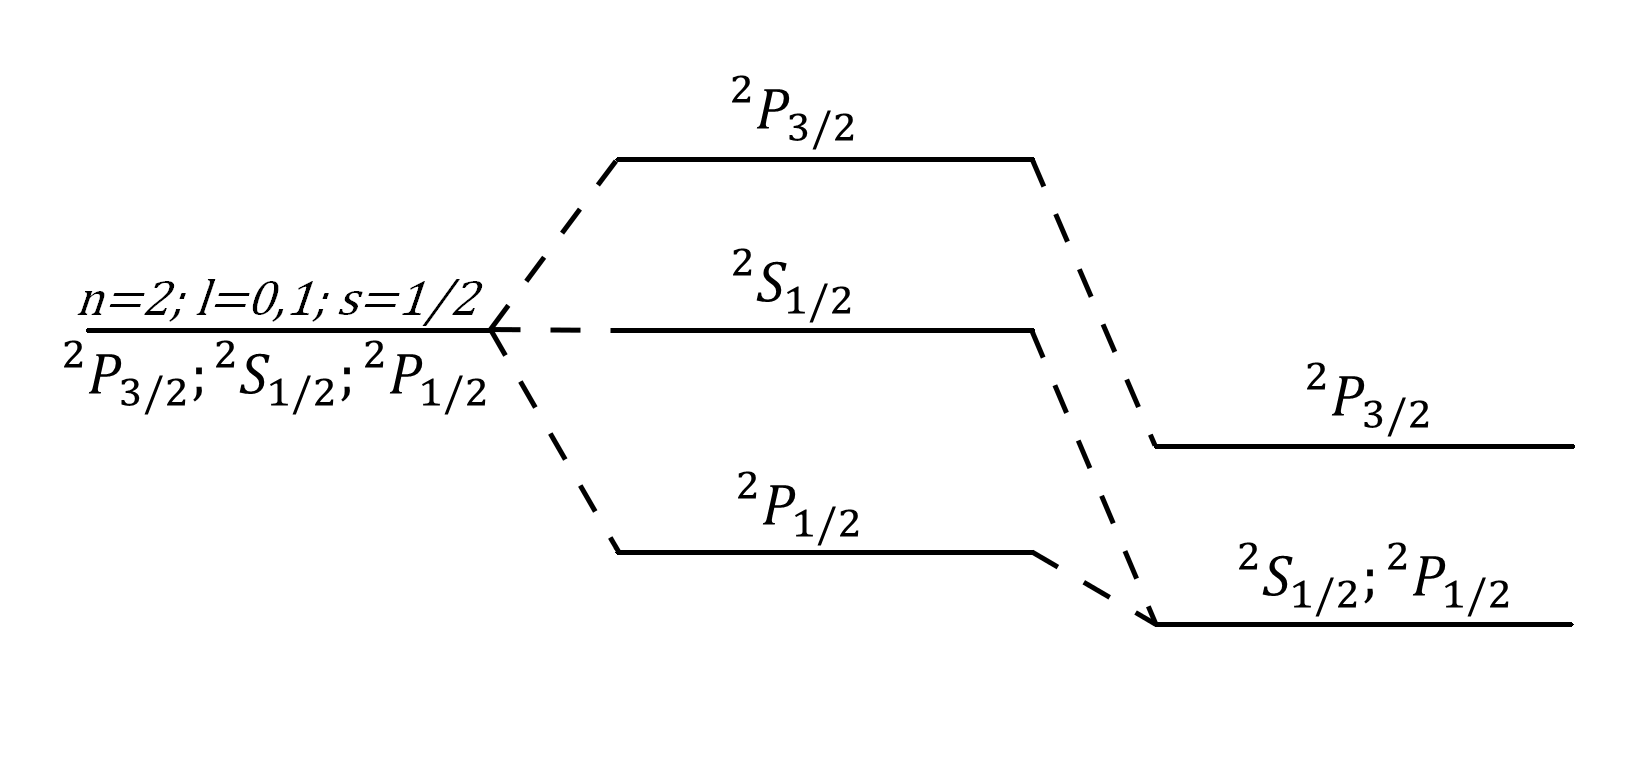
\includegraphics[width=10cm]{immagini/cap_25/fig25_1.png}
\end{center}
Gli stati con $l=1$ (stati $p$) possono avere $j=1/2$ e $j=3/2$ mentre gli stati con $l=0$ (stati $s$) corrispondono necessariamente a $j=1/2$. \'E interessante osservare le correzioni dovute allo spin-orbita e al termine cinetico si sommano in modo tale da rendere degeneri gli stati $^2S_{1/2}$ e $^2P_{1/2}$.
Una trattazione più accurata, basata sull'equazione relativistica di Dirac, non altera questo risultato. Tuttavia, nel $1947$, un accurato esperimento condotto da Lamb e Rutherford ha mostrato una sottile separazione tra i due livelli $^2S_{1/2}$ e $^2P_{1/2}$ (\textbf{Lamb-shift}). Questo effetto è spiegabile soltanto nel contesto della completa teoria quantistica relativistica ed è originato dalle fluttuazioni quantistiche del campo dell'elettrone.

\end{document}